\chapter{Durchführung}

\section{Versuchsaufbau}
Das mathematische Pendel besteht aus einer Kugel, die an einem dünnen Faden befestigt ist und an einer höhenverstellbaren Aufhängung frei schwingen kann. Zur präzisen Bestimmung der Pendellänge wurde eine vertikale Spiegelskala parallel zum Faden angebracht. Mithilfe von Nivellierschrauben konnte die Skala justiert werden, sodass der Faden in allen Aufhängungspositionen senkrecht verlief. Für die Messung der Auslenkung und zur späteren Bestimmung der Dämpfungskonstanten $\delta$ kam zusätzlich eine horizontale Spiegelskala zum Einsatz. 

Zur Bestimmung langer Periodendauern wurde eine Reflexlichtschranke direkt unterhalb der Gleichgewichtslage der Kugel angebracht. Der Sensor war so eingestellt, dass er bei jedem Durchgang der Kugel ein Signal erzeugte, welches von einem elektronischen Zähler registriert wurde. Da der Zähler bei jedem Durchgang um eins erhöht wurde, entsprach der angezeigte Wert der doppelten Anzahl von Perioden. Dies wurde bei der Auswertung entsprechend berücksichtigt. 

Vor Beginn der Messungen wurden außerdem geometrische Größen wie der Kugelradius $r$ mithilfe eines Messschiebers bestimmt, um die Trägheitsmomente nach \hyperref[eq:J]{Gleichung \ref*{eq:J}} sowie Korrekturterme in den Formeln für die Schwingungsdauer (\hyperref[eq:T_korr1]{Gleichung \ref*{eq:T_korr1}} und \hyperref[eq:T_gesamt]{Gleichung \ref*{eq:T_gesamt}}) berücksichtigen zu können.
\begin{figure}[!ht]
    \centering
    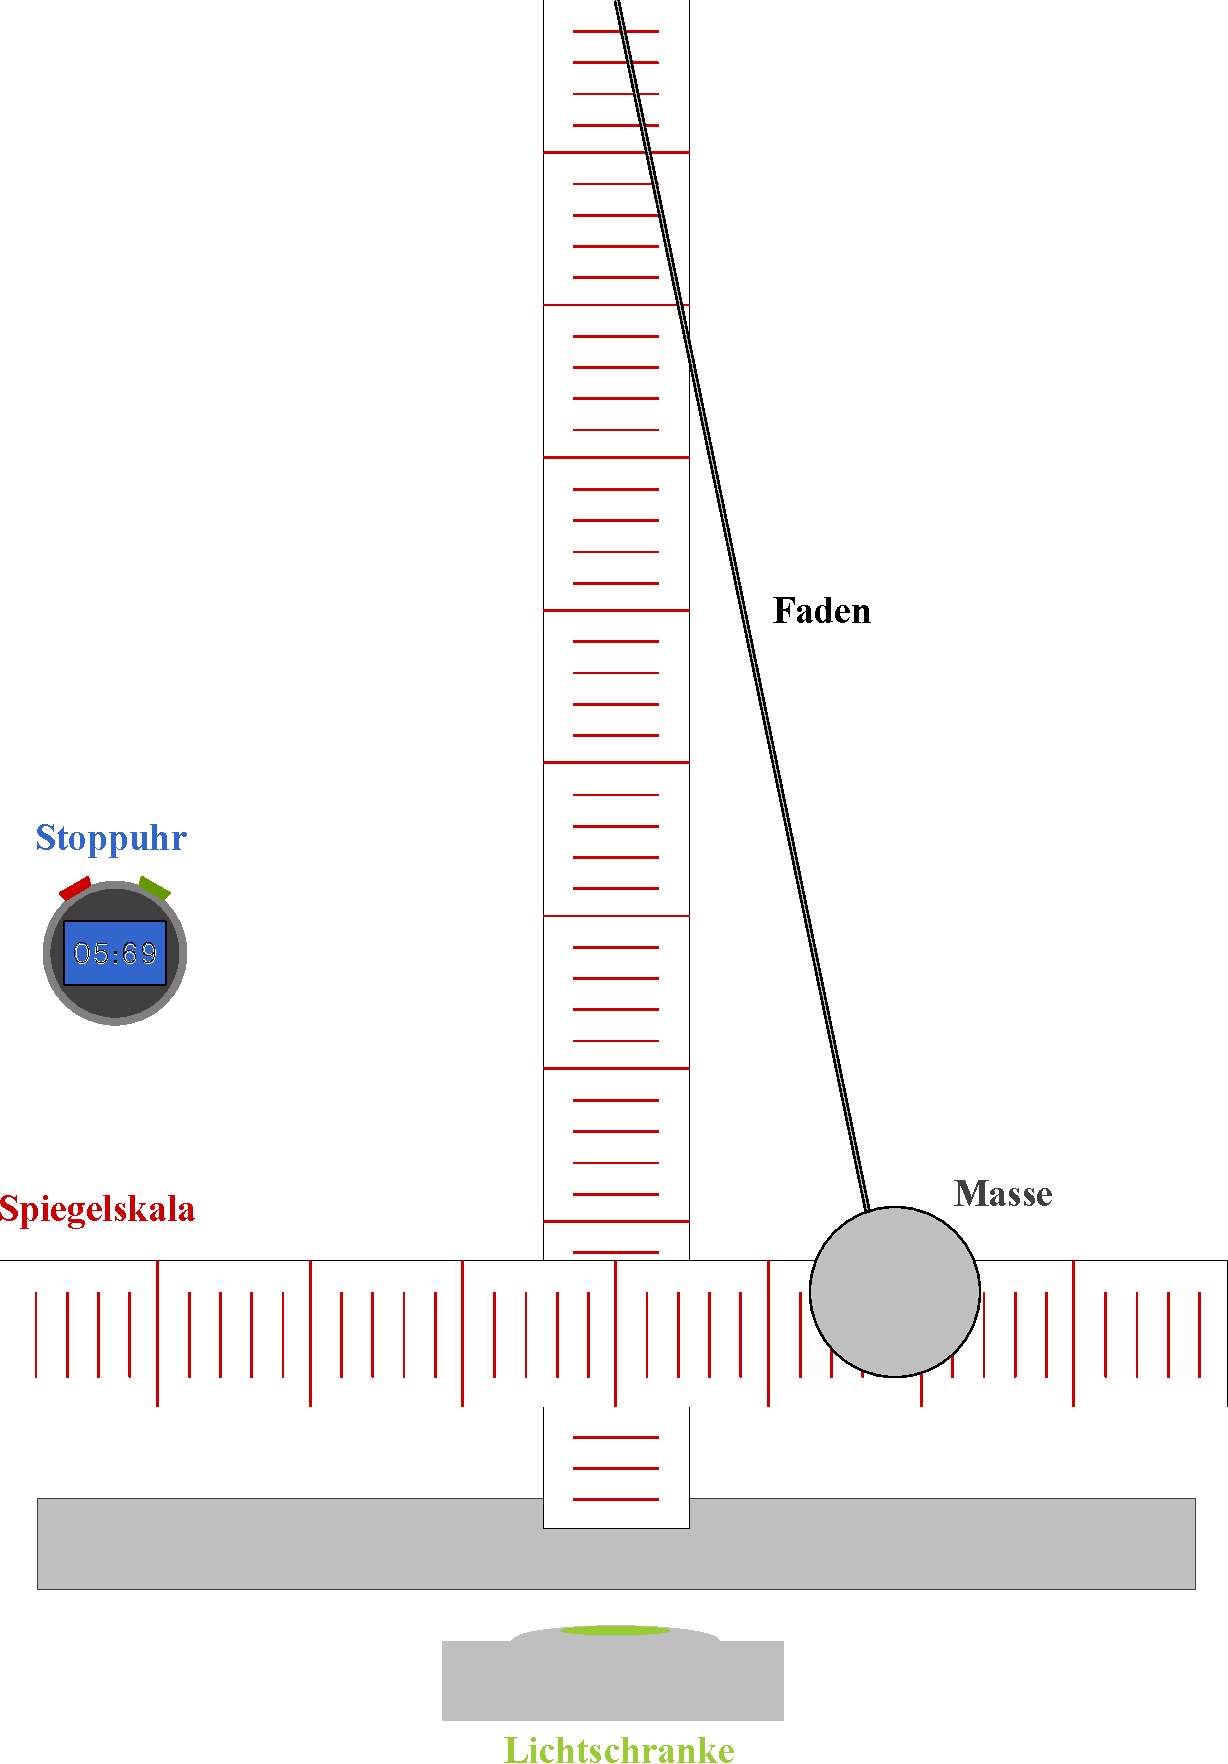
\includegraphics[width=0.45\textwidth]{img/14/Versuchsaubau.pdf}
    \caption{Schematische Versucshanordnung und Versuchsequipment.}
\end{figure}

\section{Messverfahren}
Zunächst wurde die Pendellänge $l$ bestimmt, die vom Aufhängepunkt bis zur Kugelmitte reicht. Hierfür wurden die Skalenwerte am Aufhängepunkt sowie an der oberen und unteren Kante der Kugel abgelesen. Die Messung wurde für drei verschiedene Höhen der Aufhängung durchgeführt. Aus den Werten konnte die Pendellänge und ihr relativer Fehler berechnet werden.

Die Periodendauer wurde in einem ersten Schritt durch Messung von 20 Schwingungen bestimmt. Diese Messung wurde fünfmal wiederholt, woraus der mittlere Fehler der Einzelmessung $\sigma_E$ als Stoppgenauigkeit $\Delta t$ gewonnen wurde. Mit dem so bestimmten mittleren Wert von $T_0$ aus \hyperref[eq:T0]{Gleichung \ref*{eq:T0}} konnte nach der Bedingung aus \hyperref[eq:bedingung_n]{Gleichung \ref*{eq:bedingung_n}} die notwendige Anzahl $n$ an zu messenden Perioden berechnet werden. Um den Einfluss von Fehlern möglichst gering zu halten, wurde die Anzahl der Perioden auf Anweisung des Tutors schließlich auf $n = 200$ festgelegt. Die Zeit für diese 200 Schwingungen wurde notiert und für die weitere Auswertung herangezogen. 

Zusätzlich wurde während der Schwingung alle 30 Sekunden die Amplitude mithilfe der horizontalen Spiegelskala abgelesen. Damit konnte im Nachhinein die Abnahme der Amplitude analysiert und die Dämpfungskonstante $\delta$ aus dem Zusammenhang
\begin{equation}
    a(t) = a_0 e^{-\delta t}
    \label{eq:amplitude}
\end{equation}
bestimmt werden. Diese geht in die Korrektur der Schwingungsdauer nach \hyperref[eq:T_daempfung]{Gleichung \ref*{eq:T_daempfung}} ein. Weiterhin wurde aus der mittleren Schwingungsweite der Anfangswinkel $\varphi_0$ berechnet, welcher in die Korrektur nach \hyperref[eq:T_winkel]{Gleichung \ref*{eq:T_winkel}} eingeht.

Die zur Auswertung notwendigen Größen $m_K$ und $m_F$ wurden aus den jeweiligen Volumina und der Dichte des Materials bestimmt. Mit diesen Größen konnten die Korrekturterme für das Trägheitsmoment und die Winkelrichtgröße nach \hyperref[eq:T_korr1]{Gleichung \ref*{eq:T_korr1}} berechnet werden. Schließlich lässt sich die Erdbeschleunigung $g$ am Versuchsort durch Einsetzen der gemessenen Werte in \hyperref[eq:T_gesamt]{Gleichung \ref*{eq:T_gesamt}} bestimmen.

